% $Id: Note_ResFit_QCDMC_Extrapolation.tex,v 1.2 2010/07/07 16:57:14 mschrode Exp $


\subsection{Extrapolation to the Two Jet Final State Topology}\label{sec:ResFit:QCDMC:Extrapolation}

As discussed in the previous Section~\ref{sec:ResFit:QCDMC:AddJetAct},
the presence of additional jets in the dijet event biases the
measurement towards larger resolutions and thus has to be corrected
for.
The size of the particle level jet \pt imbalance is correlated with the
measured relative \pt of the third jet as illustrated in Fig.~\ref{}.
Hence, in order to compensate for the bias in a data driven manner, different dijet samples with different maximal values $x$ of \ptrel (comp. step~1 of the event selection, Section~\ref{sec:ResFit:QCDMC:EvtSel}) are selected and the maximum likelihood fit is performed each time.
Then, the resulting resolution is extrapolated to the case of a two jet only event i.e. \mbox{$\ptrel\rightarrow0$}.

The approach chosen in the following is to define sufficiently small bins of jet \pt and measure the w.r.t. \pt average response in each bin for different limits \mbox{$\ptrel<x$}.
This is motivated by the fact that in case of a Gaussian response parametrisation (Section~\ref{sec:ResFit:QCDMC:Gauss}) there is then only one parameter $\bar{\sigma}$, which can be extrapolated relatively straight forward.
The chosen \pt and $\eta$ binning is listed in Table~\ref{tab:ResFit:QCDMC:Extrapolation:Binning}.
\begin{table}[ht]
  \caption{Definition of \pt bins for the fit of the mean Gaussian resolution.}
  \centering
  \begin{tabular}{cl|ccccccccc}
    \toprule
    \multicolumn{2}{c}{$|\eta|$ bin} & \multicolumn{9}{c}{\pt bin edges $(\text{Ge}\kern-0.06667em\text{V})$} \\
    \midrule
    \multirow{2}{*}{$0$} & \multirow{2}{*}{$(0 - 1.2)$} & 80 & 100 & 120 & 140 & 170 & 200 & 250 & 300 & 350 \\
    && 400 & 500 & 600 & 800 & 1000 \\
    $1$ & $(1.2 - 2.6)$ & 60 & 80 & 100 & 120 & 150 & 200 & 300 &  500 & 700 \\
    $2$ & $(2.6 - 3.2)$ & 80 & 100 & 150 &&&&&&\\
    \bottomrule
  \end{tabular}
  \label{tab:ResFit:QCDMC:Extrapolation:Binning}
\end{table}

Was the Gaussian parametrised with a \pt dependent $\sigma$ as e.g. in~\eqref{eq:ResFit:ToyMC:Sigma}, the correlation of the parameter $\xi_{i}$ of $\sigma$ would have to be taken into account in contrast.
Note that this is exactly the case for the Crystal Ball response parametrisation (Section~\ref{sec:ResFit:QCDMC:CrystalBall}), and additional work is forseen to uncorrelate the parameters $\sigma$, $\alpha$, and $n$.

In the following, the particle level differential dijet cross section is taken from the interpolated \ptparticle distribution Fig.~\ref{fig:ResFit:QCDMC:Extrapolation:Gauss:ExBin:SpectrumAndExtrapolation} (\textit{left}) that has been obtained from the Monte Carlo truth information. 



\subsubsection{Measurement of the Gaussian response function}\label{sec:ResFit:QCDMC:Gauss}

A sample of dijet events is selected for each $\eta$, \pt bin listed in Table~\ref{tab:ResFit:QCDMC:Extrapolation:Binning}.
The selection bias (Section~\ref{sec:ResFit:Method:Biases}) is incorporated in the probability densitity function as before, comp. Fig.~\ref{fig:ResFit:QCDMC:Extrapolation:Gauss:ExBin:SpectrumAndExtrapolation} (\textit{left}).

\begin{figure}[ht]
  \centering
  \begin{tabular}{cc}
    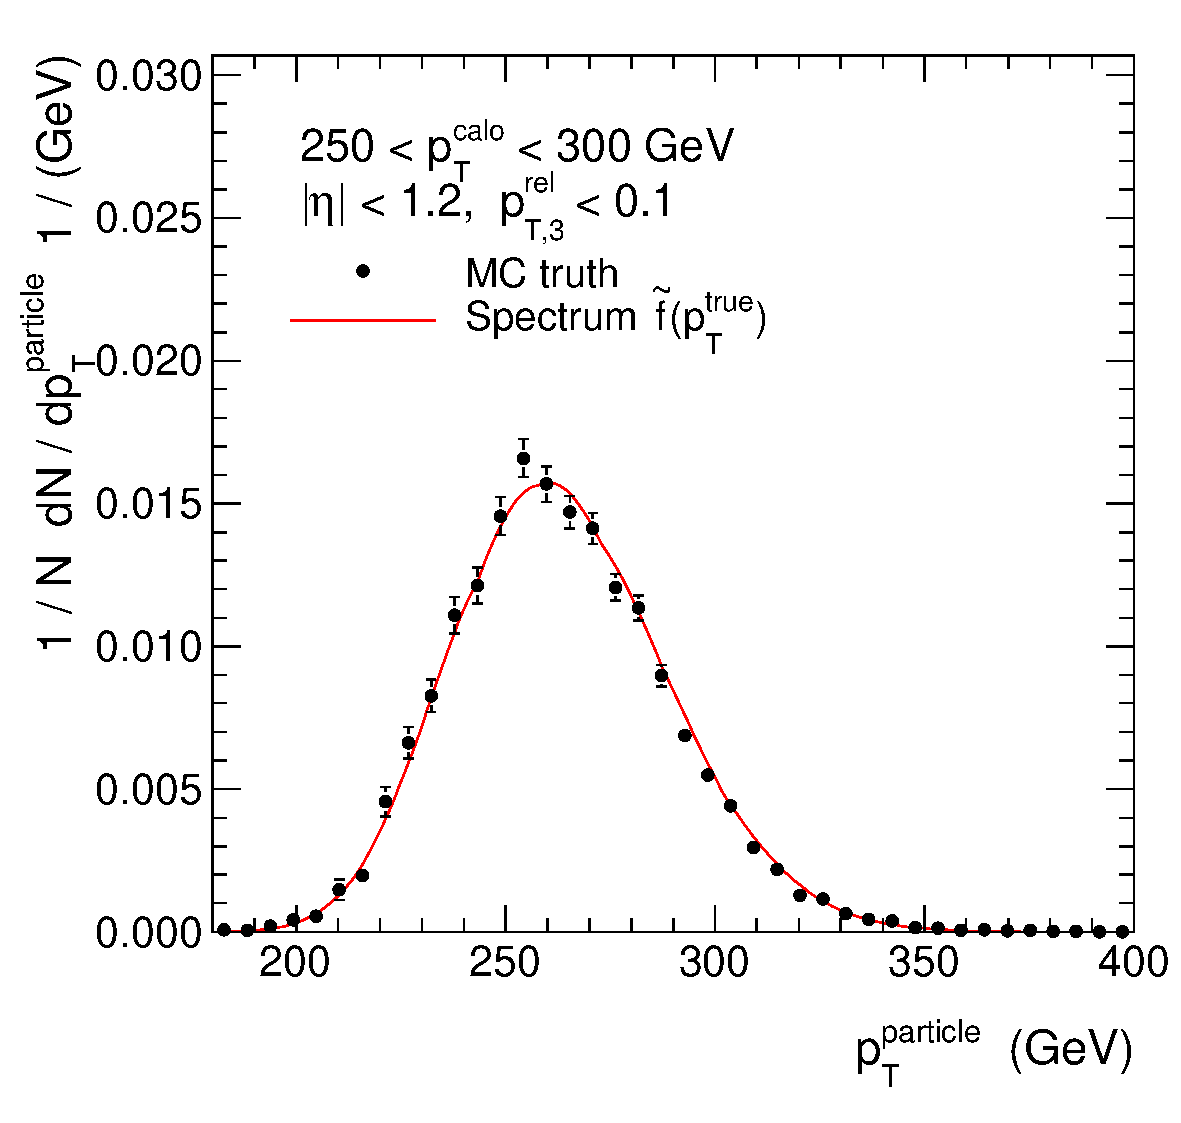
\includegraphics[width=0.45\textwidth]{figures/ResFit_Spring10QCDFlat_Gauss_Eta0_Spectrum_PtBin6} &
    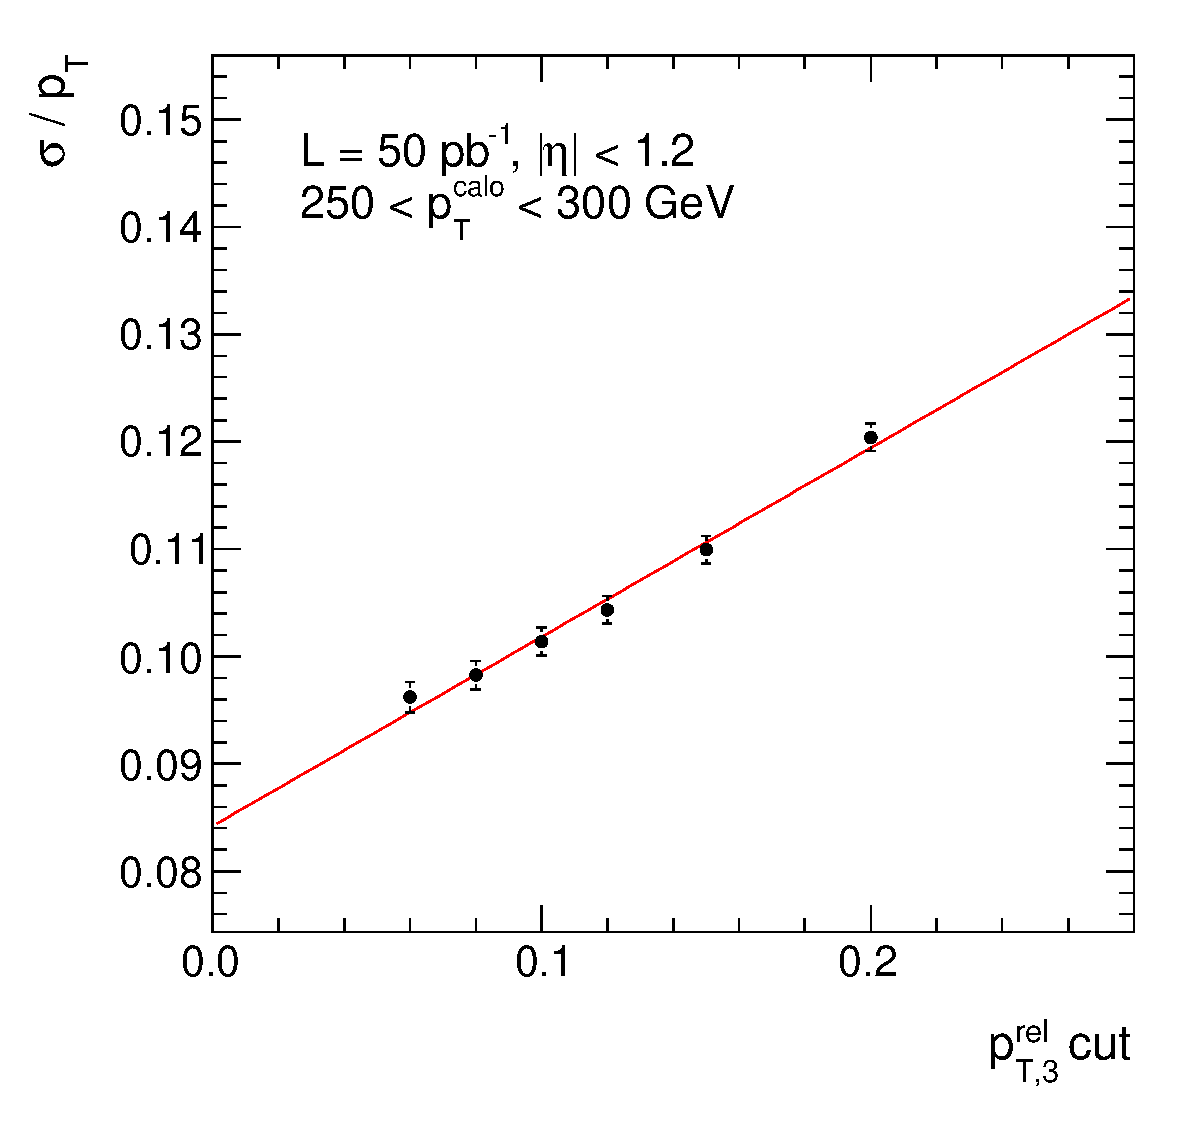
\includegraphics[width=0.45\textwidth]{figures/ResFit_Spring10QCDFlat_Gauss_Eta0_ExtrapolatedPar0_PtBin6}
  \end{tabular}
\caption{(\textit{Left}) The parameterisation of the realistic particle jet \pt spectrum in one \pt bin as used in the dijet likelihood (solid line) in comparison to the prediction from Monte Carlo truth (full circles). 
  (\textit{Right}) $\bar{\sigma}/\pt$ from Gaussian fits for different limits on \ptrel in the same \pt bin.
  The solid line is a linear fit to extrapolate $\bar{\sigma}/\pt$ to the ideal case of only two jets in the
  final state.}
\label{fig:ResFit:QCDMC:Extrapolation:Gauss:ExBin:SpectrumAndExtrapolation}
\end{figure}

The mean Gaussian response
\begin{equation*}
  r_{\mathbf{\bar{\sigma}}}\left(\ptmeas|\pttrue\right) = 
  \frac{1}{\sqrt{2\pi}\bar{\sigma}}\exp\left[-\frac{1}{2}\left(\frac{\ptmeas - \pttrue}{\bar{\sigma}}\right)^{2}\right]
\end{equation*}
is measured in each bin by maximising the likelihood~\eqref{eq:ResFit:Likelihood} w.r.t.~$\bar{\sigma}$.
The fitted relative Gaussian widths $\bar{\sigma}/\pt$ in one \pt bin are shown in Fig.~\ref{fig:ResFit:QCDMC:Extrapolation:Gauss:ExBin:SpectrumAndExtrapolation} (\textit{right}) for different limits on \ptrel.
Here, \pt is the mean value of the asssumed spectrum~$\tilde{f}(\pttrue)$ in that bin, shown Fig.~\ref{fig:ResFit:QCDMC:Extrapolation:Gauss:ExBin:SpectrumAndExtrapolation} (\textit{left}).
In order to extrapolate the measurements to the case of a two jet only event, the $\bar{\sigma}/\pt$ are fitted with a linear function --- shown as a solid line --- and the $y$ axis intercept is taken as the corrected jet \pt resolution.

The jet \pt spectra, fitted Gaussian resolutions $\bar{\sigma}/\pt$ versus \ptrel, and the extrapolation are shown in Appendix~\ref{sec:ResFit:App:Gauss:AllResults} for all \pt and $\eta$ bins.

\begin{figure}[ht]
  \centering
  \begin{tabular}{cc}
    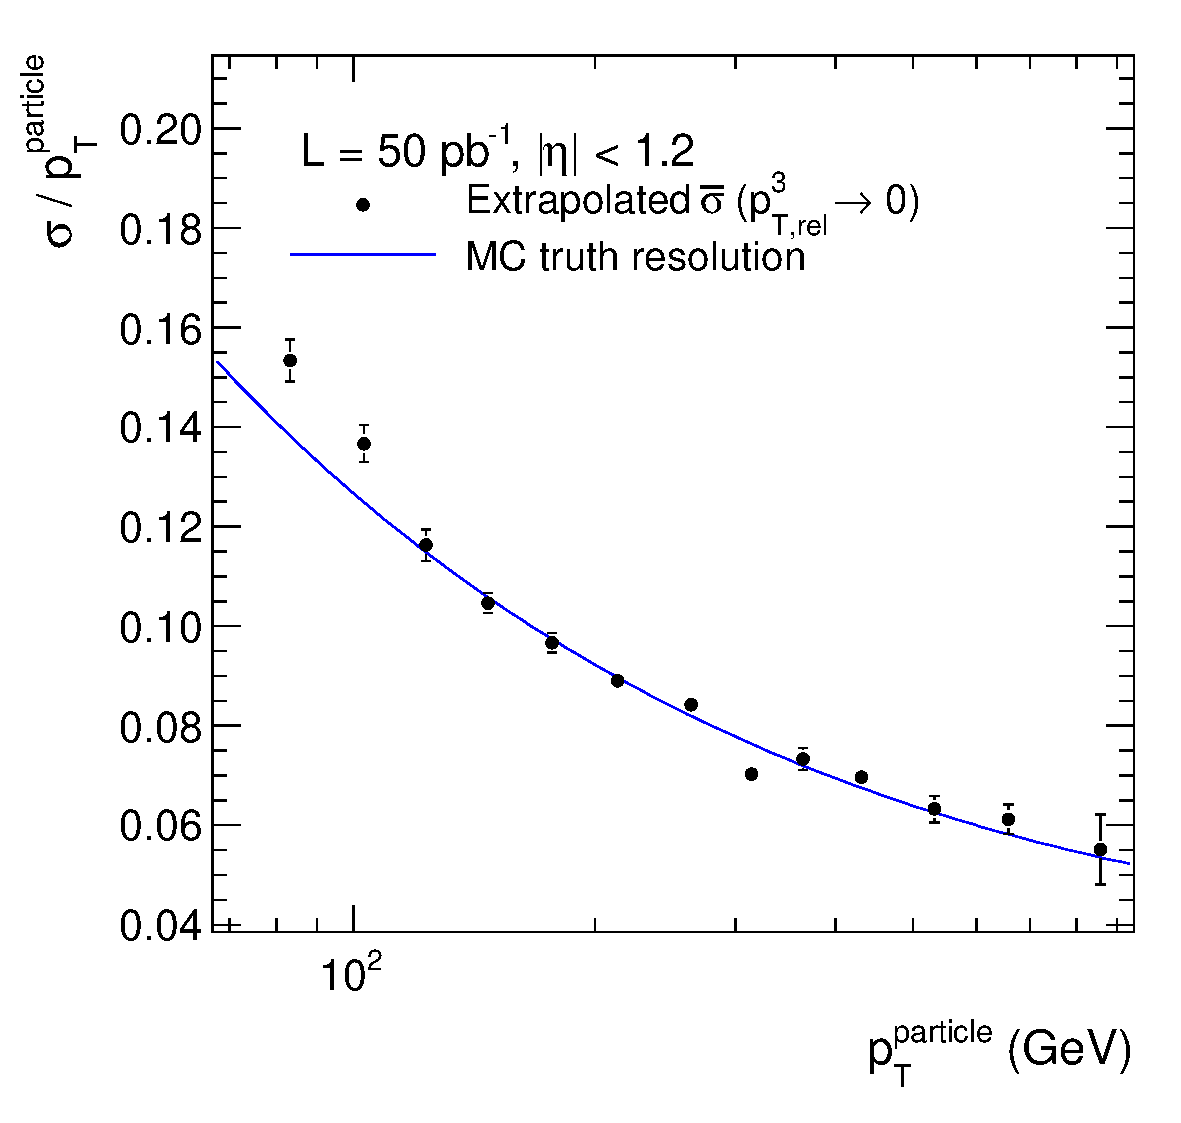
\includegraphics[width=0.45\textwidth]{figures/ResFit_Spring10QCDFlat_Gauss_Eta0_ExtrapolatedResolution} &
    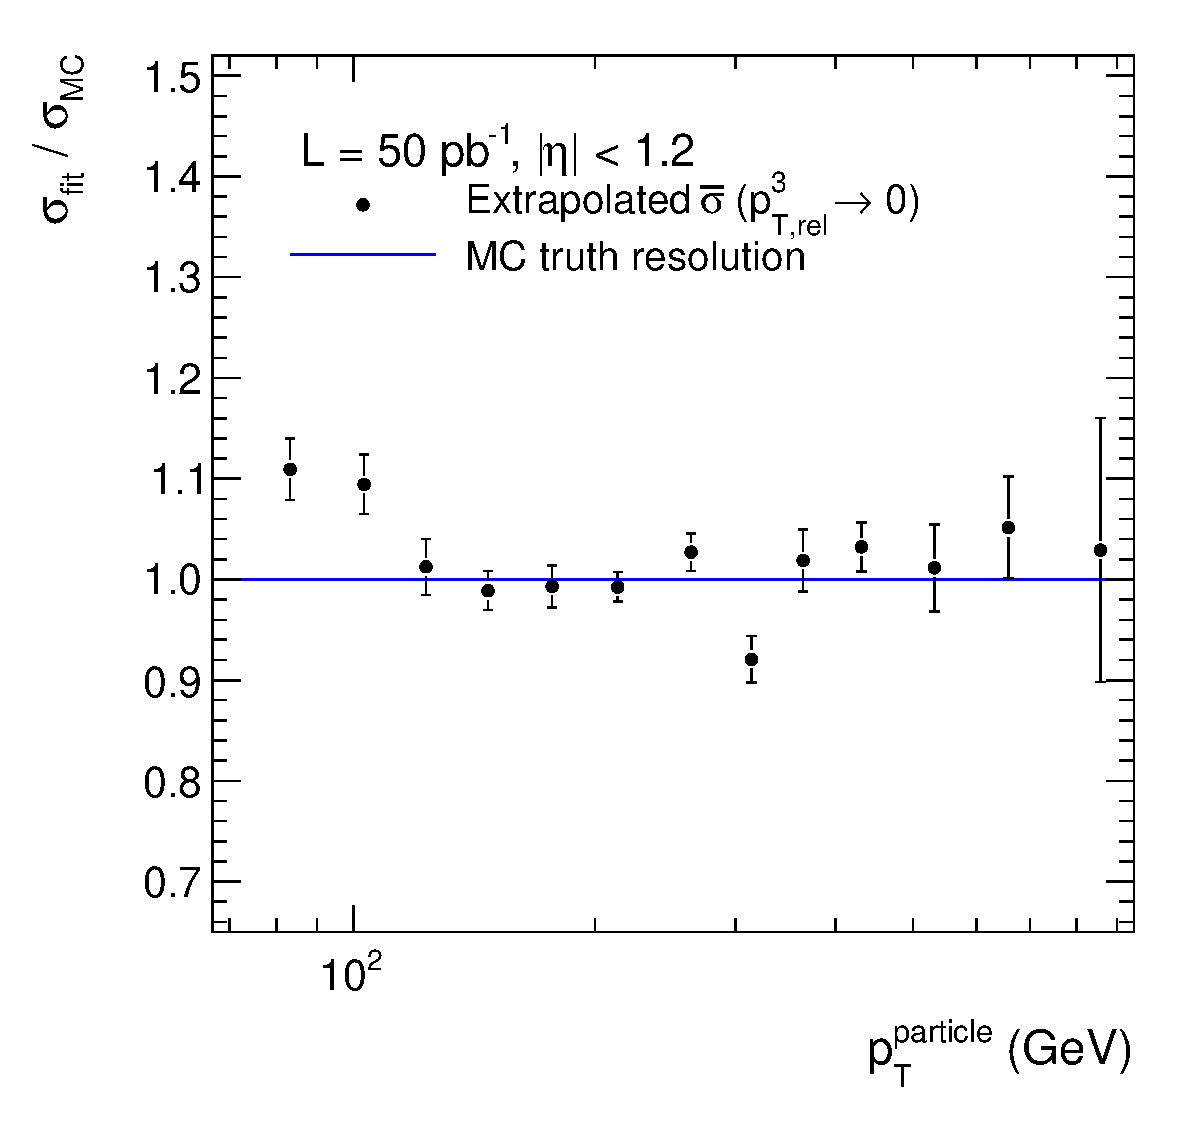
\includegraphics[width=0.45\textwidth]{figures/ResFit_Spring10QCDFlat_Gauss_Eta0_ExtrapolatedResolutionRatio}
  \end{tabular}
\caption{(\textit{Left}) Fitted Gaussian jet \pt resolutions, $\bar{\sigma}/\pt$, from extrapolations for \mbox{$\ptrel\rightarrow0$} in different \pt bins.
  The \pt are the mean values of $\tilde{f}(\pttrue)$ in each bin.
  The error bars indicate the combined statistical uncertainties from the extrapolation and the Monte Carlo statistics.
  The dashed line shows the Monte Calro truth resolution for comparison.
  (\textit{Right}) Ratio of fitted and Monte Carlo truth resolution.}
\label{fig:ResFit:QCDMC:Extrapolation:Gauss:ResoVsPt}
\end{figure}

The jet \pt resolution $\bar{\sigma}/\pt$ measurements, corrected for the effect of additional jet activity, are shown for different \pt bins in Fig.~\ref{fig:ResFit:QCDMC:Extrapolation:Gauss:ResoVsPt}.
(Again, the \pt are the mean values of the asssumed spectrum~$\tilde{f}(\pttrue)$ in each bin.)
The fitted values are in good agreement with the Monte Carlo truth prediction, shown as a dash line.
The larger deviation in the two low \pt bins is assumed to be caused by the increasing influence of incorrect jet ordering due to the greater resolution on the extrapolation procedure\footnote{This effect is seen when using the dijet asymmetry method to measure jet \pt resolutions~\cite{bib:cmspas:dijetasymm}.}.

The error bars shown in Fig.~\ref{fig:ResFit:QCDMC:Extrapolation:Gauss:ResoVsPt} represent the combined statistical uncertainties of the fit and due to the Monte Carlo sample size:
\begin{enumerate}
\item The first contribution is the statistical uncertainty on the parameter of $y$ axis intercept in the linear extrapolation (Fig.~\ref{fig:ResFit:QCDMC:Extrapolation:Gauss:ExBin:SpectrumAndExtrapolation} (\textit{left})).
\item The second contribution arises from the uncertainty due to the limited Monte Carlo sample size.
 As the event weights are large for small \pt, statistical fluctations become significant.
 In order to roughly evaluate this uncertainty, the same fits have been performed again without event weights (for the used sample this corresponds to a flattened QCD spectrum).
 The statistical uncertainties obtained in this case on the $y$ axis intercept are added in quadrature to the ones in 1.
 This procedure has to be improved to obtain a statistically correct description of the uncertainty.
\end{enumerate}

Due to the selection requirement \mbox{$\ptrel < x$}, all events selected for a particular value of $x$ in Fig.~\ref{fig:ResFit:QCDMC:Extrapolation:Gauss:ExBin:SpectrumAndExtrapolation} (\textit{right}) are also included in the samples selected with larger values of $x$.
Hence, the measured widths $\bar{\sigma}/\pt$ in one \pt are strongly correlated.
This correlation is not considered in the qouted uncertainties.
The planned treatment is to either include the correlations explicitly or performe the measurements in exclusive bins of \ptrel.

\begin{figure}[ht]
  \centering
    \begin{tabular}{ccc}
      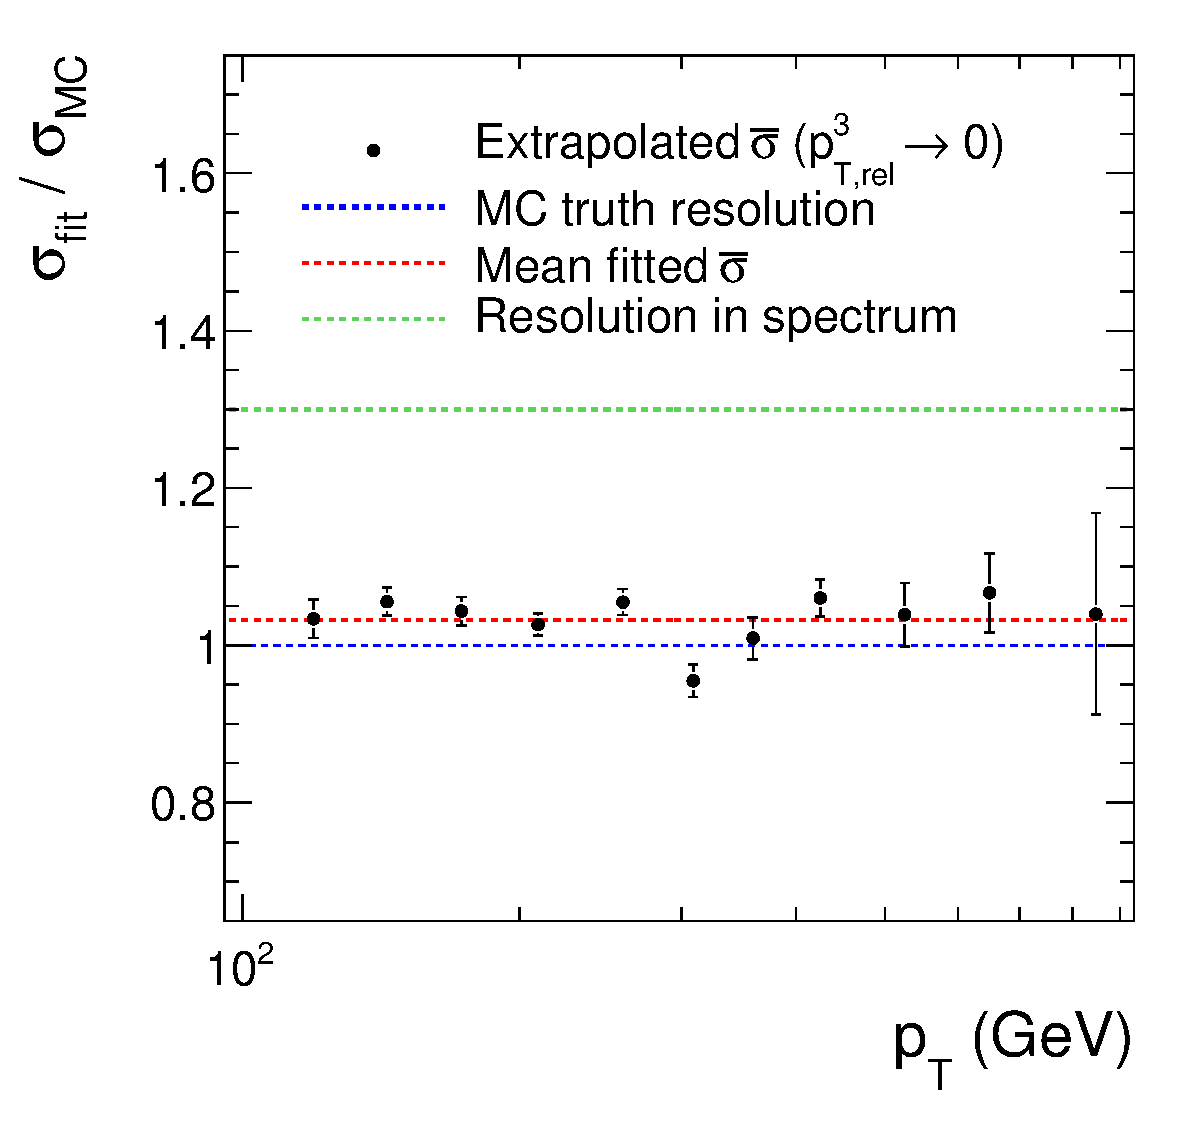
\includegraphics[width=0.3\textwidth]{figures/ResFit_Spring10QCDFlat_GaussUp30It0_Eta0_ExtrapolatedResolutionRatio} &
      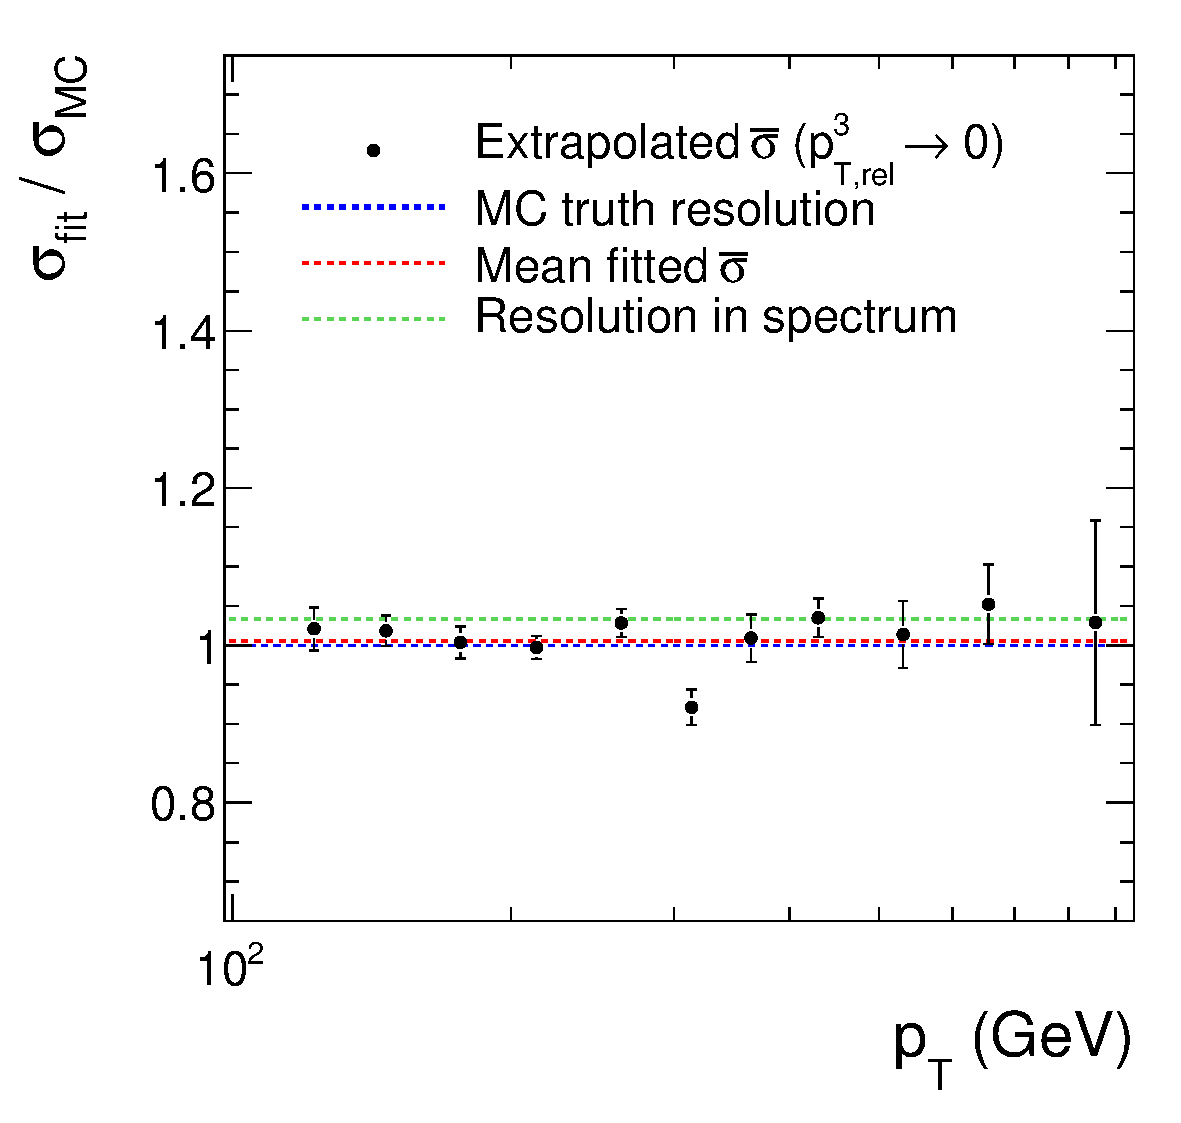
\includegraphics[width=0.3\textwidth]{figures/ResFit_Spring10QCDFlat_GaussUp30It1_Eta0_ExtrapolatedResolutionRatio} &
      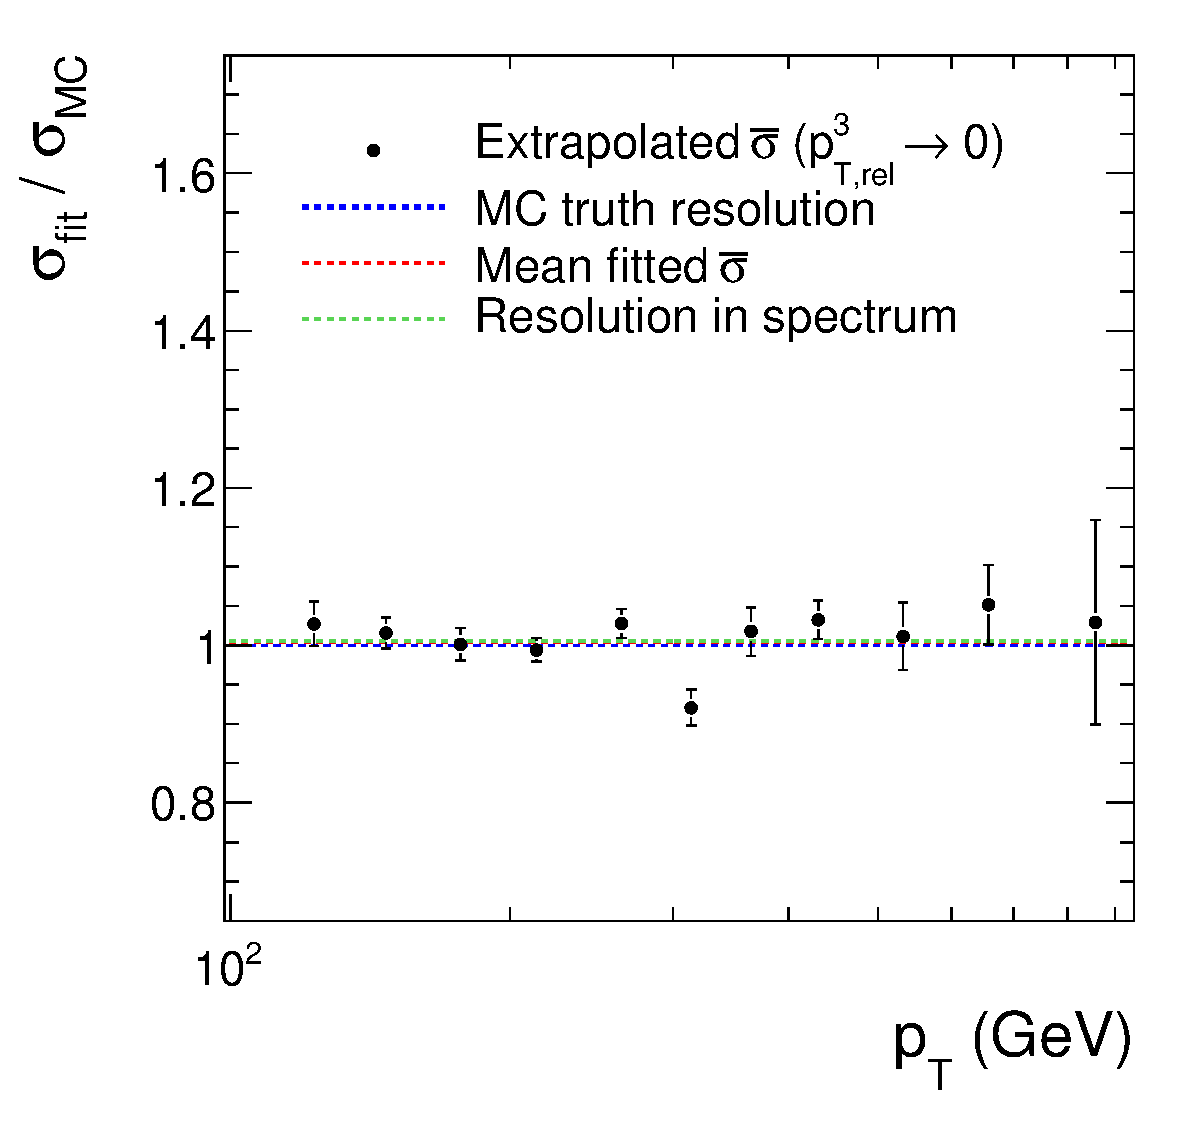
\includegraphics[width=0.3\textwidth]{figures/ResFit_Spring10QCDFlat_GaussUp30It2_Eta0_ExtrapolatedResolutionRatio}
    \end{tabular}
  \caption{The solid black markers show the measured Gaussian jet \pt resolutions in different \pt bins.
  The dashed green line is the assumed resolution to describe the selection bias during the fit.
  The dashed red line corresponds to the average measured resolution.
  Actually shown is the ratio to the Monte Carlo truth resolution in all cases.
  (\textit{Left}) The assumed resolution deviates by $30\%$ from the truth, the measured resolution by only $3.3\%$.
  (\textit{Centre}), (\textit{right}) The measured resolution from the previous iteration is taken as assumed resolution during the fit.
  The plots demonstrate the stability of an iterative procedure.}
  \label{fig:ResFig:QCD:Extrapolation:Gauss:Iterations}
\end{figure}

A description of the selection bias has been incorporated into the dijet probability density by assuming a jet \pt response $r_{0}(x|\pttrue)$ (Section~\ref{sec:ResFit:Method:Biases}).
In order to evaluate the influence of $r_{0}$ on the measured resolution, the fit has been performed with $r_{0}$ varied by $+30\%$ i.e. $\sigma_{0}\rightarrow 1.3\sigma_{0}$ (Fig.~\ref{fig:ResFig:QCD:Extrapolation:Gauss:Iterations}~\textit{left}).
The measured resolution deviates by $+(3.3 \pm 0.7)\%$ on average, demonstrating the weak influence of $r_{0}$ on the result.
A second and a third measurement have been performed, each time with the result of the previous as input for $r_{0}$, leading to decreasing average deviations (comp. Fig~\ref{fig:ResFig:QCD:Extrapolation:Gauss:Iterations} \textit{centre}, \textit{right}).
Hence, an iterative procedure is applicable. 



\subsubsection{Measurement of the full response function}\label{sec:ResFit:QCDMC:CrystalBall}
